%\ctparttext{\color{black}\begin{center}
%		Esta es una descripción de la parte de informática.
%\end{center}}

%\part{Parte de informática}
\chapter{Caso 2: Comparación de rentas}


\section{Descripción del caso de estudio}
Este caso de estudio trata de contrastar las diferencias que hay entre grupos con renta baja (menor de $15000$€ al año) y renta alta (mayor de $25000$€ al año).

Para ello, las variables seleccionas son:
\begin{itemize}
\item \textbf{Renta}: Renta disponible total del hogar en el año anterior al de encuesta.
\item \textbf{Alimentos}: Durante el mes pasado, ¿cuál fue aproximadamente el importe que el hogar gastó en alimentos y bebidas no alcohólicas para ser consumidas en casa?
\item \textbf{Asistencia social}: Ingresos por asistencia social en el año anterior al
de encuesta.
\item \textbf{Gastos}: Gastos de la vivienda: Alquiler (si la vivienda se encuentra en régimen de alquiler), intereses de la hipoteca (para viviendas en propiedad con pagos pendientes) y otros gastos asociados (comunidad, agua, electricidad, gas, etc.)
\end{itemize}

Para realizar la comparativa, vamos a estudiar dos subcasos, el primero con renta baja y el segundo con renta alta.

\section{Caso 2 A: Renta baja}

Este caso de estudio consta de $3197$ elementos, cada uno con las cuatro variables especificadas antes.

\subsection{Ejecución de algoritmos}

Ejecutamos la celda del notebook de jupyter correspondiente al caso 2A (que se puede configurar para sacar las distintas gráficas) y obtenemos así las diferentes medidas obtenidas para cada algoritmo, que se muestran en \eqref{tab:c2A_alg}.

\begin{table}[H]
\centering
\caption{Caso 2A - Resultados de ejecución de algoritmos.}
\label{tab:c2_alg}
\begin{tabular}{ccccc}
\toprule
 Algoritmo & Tiempo (s) & Silhouette & Calinski-Harabasz & Número de clusters \\
\midrule
kmeans & 0.385 & 1157.588 & 0.31325 & 5 \\
birch & 0.124 & 510.565 & 0.26449 & 5 \\
spectral & 1.739 & 1068.474 & 0.30286 & 5 \\
dbscan & 0.171 & 304.282 & 0.60850 & 2 \\
meanshift & 18.233 & 184.067 & 0.40807 & 11 \\
\bottomrule
\end{tabular}
\end{table}

Respecto a los tiempos, de nuevo el algoritmo más lento es meanshift, seguido de spectral cluster. El resto de algoritmos obtienen tiempo similares.

Además, al igual que en el caso 1 DBSCAN ha generado solamente dos clusters, uno con el $97.12\%$ de los datos y los restantes en el cluster -1.Meanshift vuelve a generar más cluster que el resto, agrupanod uno de ellos al $91.46\%$ de elementos, otro al $4.86\%$ y el resto cada uno contiene un número de elementos menor al $1.2\%$ del total. Por ello, parece que a pesar de las medidas que han obtenido, estos algoritmos no han realizado un buen agrupamiento.

Finalmente vemos como Birch tiene un valor de Calinski-Harabasz y silhouette más bajo que kmeans y spectral cluster. Estos algoritmos han conseguido medidas similares, obteniendo en principio kmeans mejores resultados.


\subsection{Análisis}


Para el análisis se va a usar kmeans, ya que ha obtenido los mejores en las medidas. Este algoritmo genera 5 clusters. Se ha generado un cluster de tamaño menor, y los otros tienen tamaños similares dos a dos, como se puede ver en \eqref{c2A_tam}.

\begin{figure}[H]
\caption{Caso 2A- Tamaño de los clusters generados por kmeans}
\label{c2A_tam}
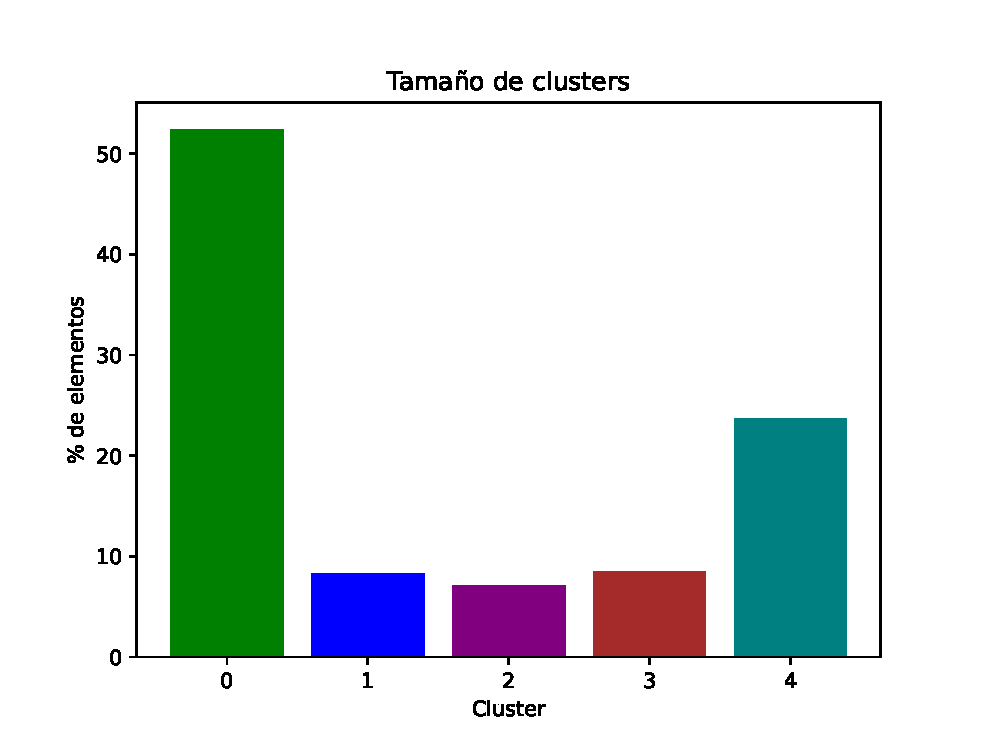
\includegraphics[scale=1]{caso2A/kmeans/bar.eps}
\end{figure}

A continuación observamos la scatter matrix \eqref{c2A_scatter}, donde se puede apreciar como se separan os clusters y qué variables son necesarias para separar cada uno. Hay varios clusters que se diferencian bien con una sola variable, como es el caso de cluster 0, que tiene valores altos de gastos, el 4 tiene valores más altos en asistencia social y el 2 gasta más en alimentación. Los clusters 1 y 3 se distinguen bien usando renta y gastos o renta y alimentos, ya que ambos tienen valores bajos de renta y uno tiene valores mayores que el otro en la variable restante.

\begin{figure}[H]
\caption{Caso 2A- Scatter matrix de kmeans}
\label{c2A_scatter}
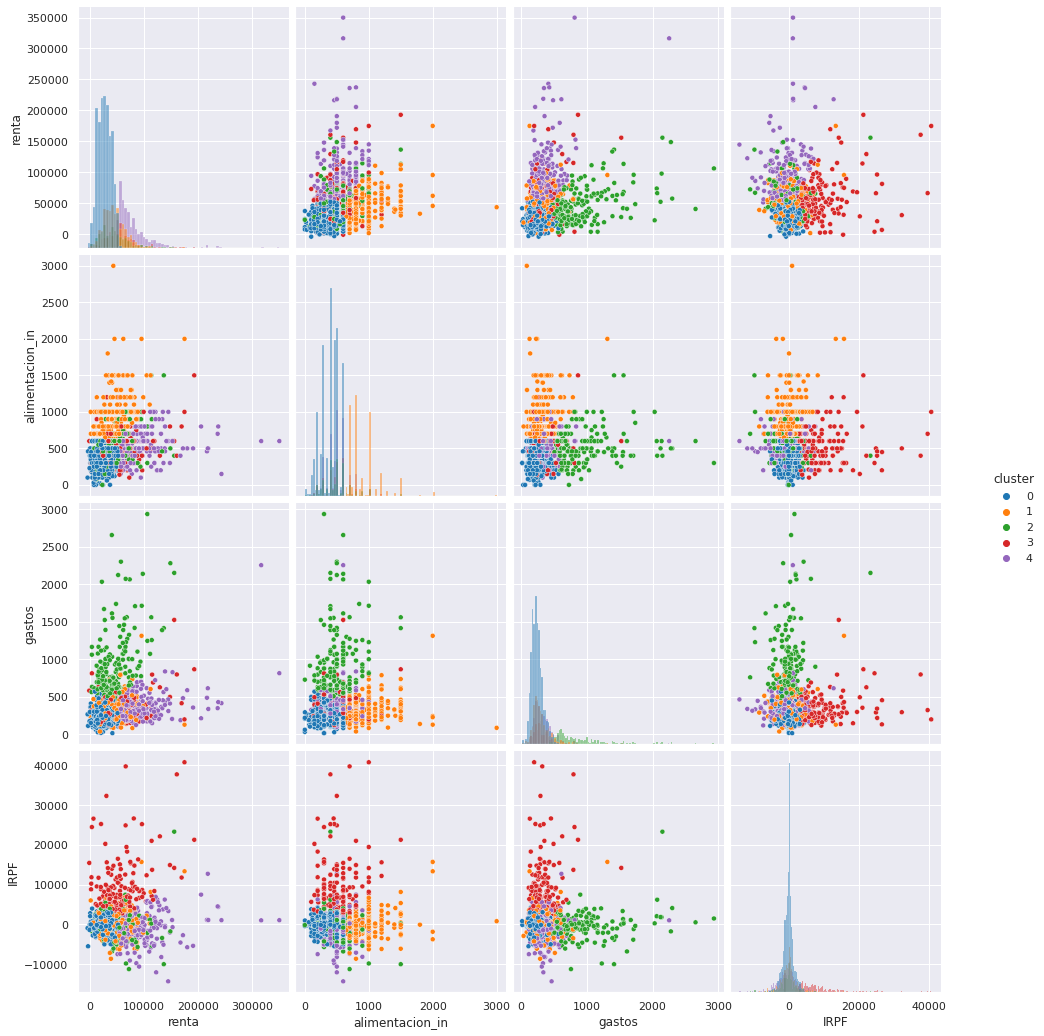
\includegraphics[scale=0.45]{caso2A/kmeans/scatter.png}
\end{figure}


\begin{figure}[H]
\caption{Caso 2A- Heatmap de kmeans}
\label{c2A_heatmap}
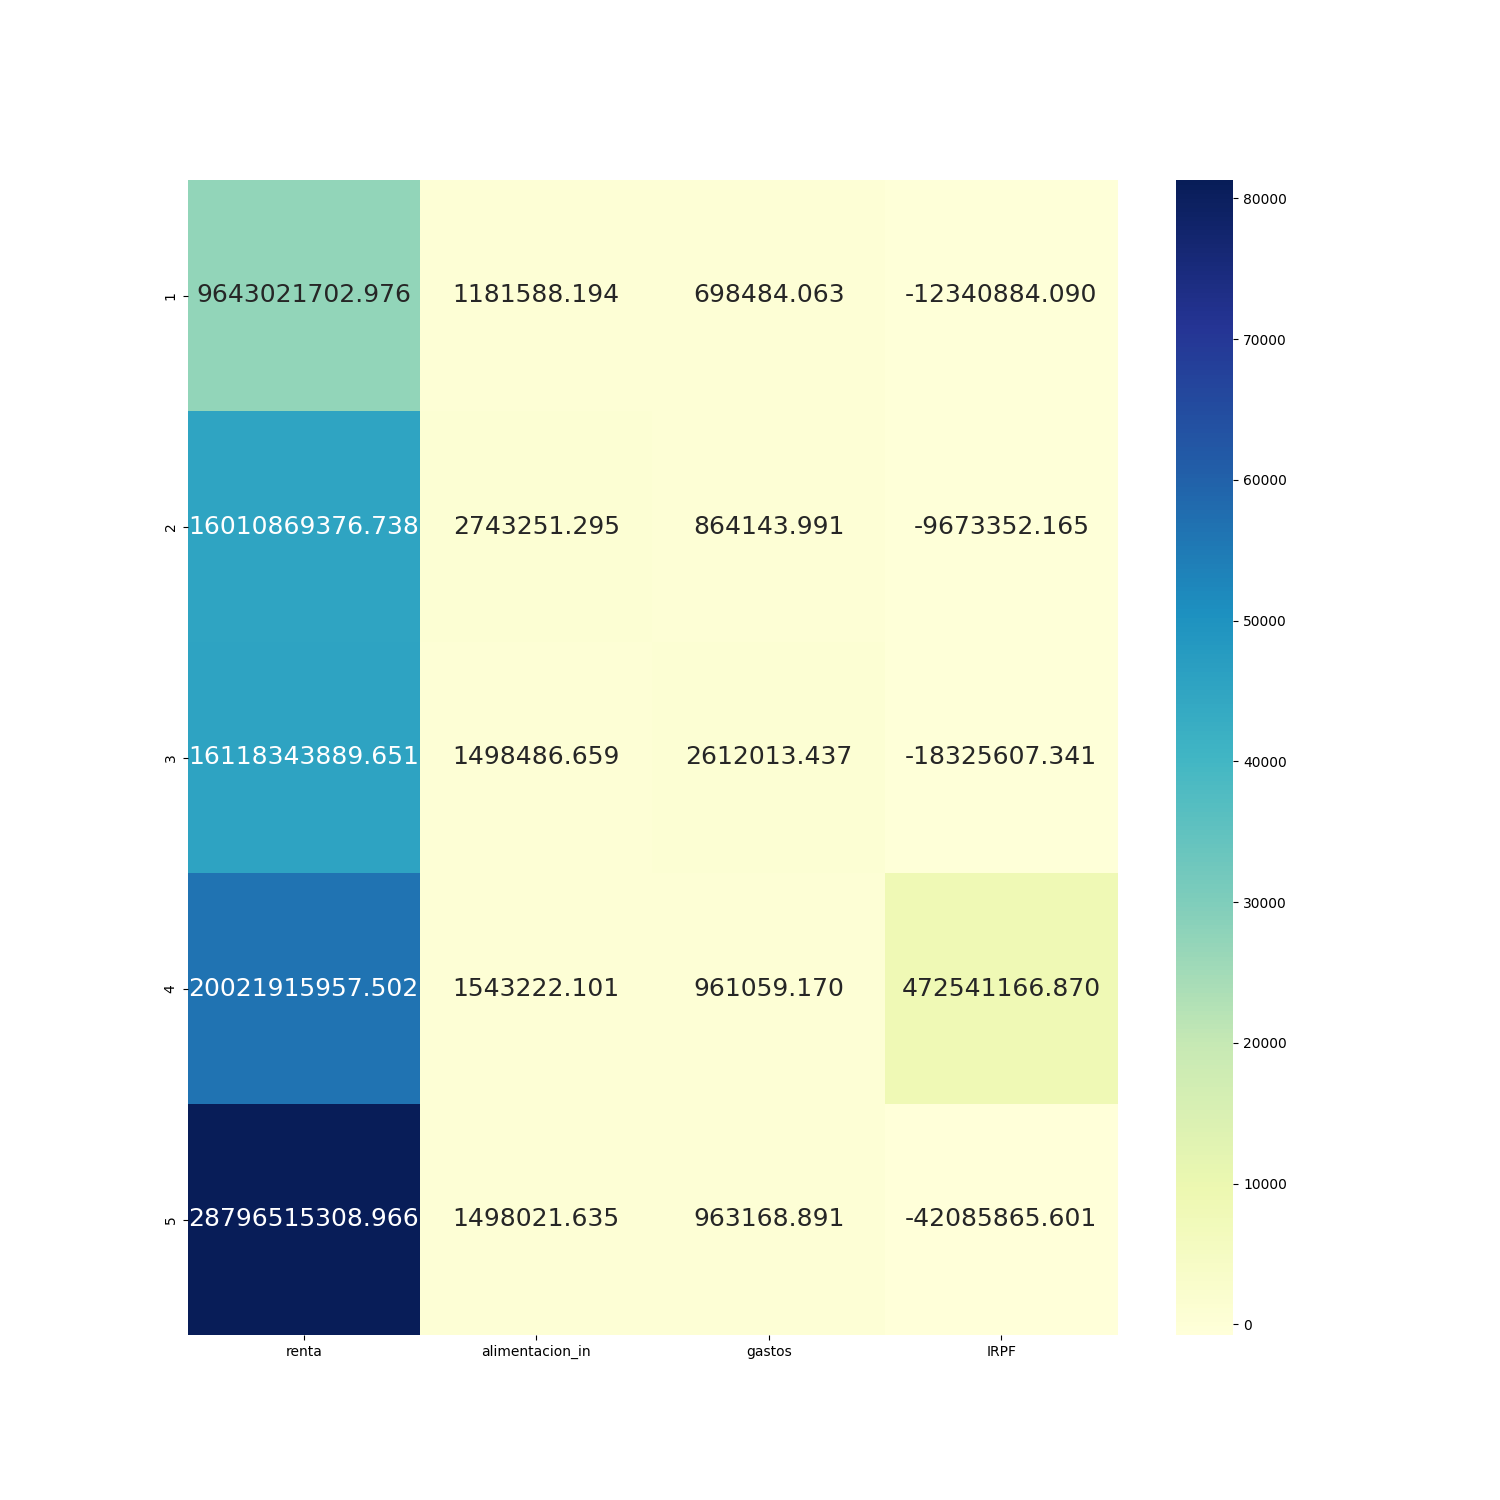
\includegraphics[scale=0.45]{caso2A/kmeans/heatmap.png}
\end{figure}

En \eqref{c2A_heatmap} se ve con claridad los tres clusters que se diferencian por tomar valores especialmente altos en una de sus variables. Teniendo en cuenta que la numeración en este gráfico va de 1 a 5 y en la scatter matrix va de 0 a 4, vemos la analogía. En el heatmap se ve con claridad como el cluster 5 toma valores considerablemente más altos en asistencia social que el resto de clusters, el 3 toma valores más altos en alimentación y el 1 en gastos, lo que concuerda con lo visto en la scatter matrix.


\begin{figure}[H]
\caption{Caso 2A- MDS de kmeans}
\label{c2A_mds}
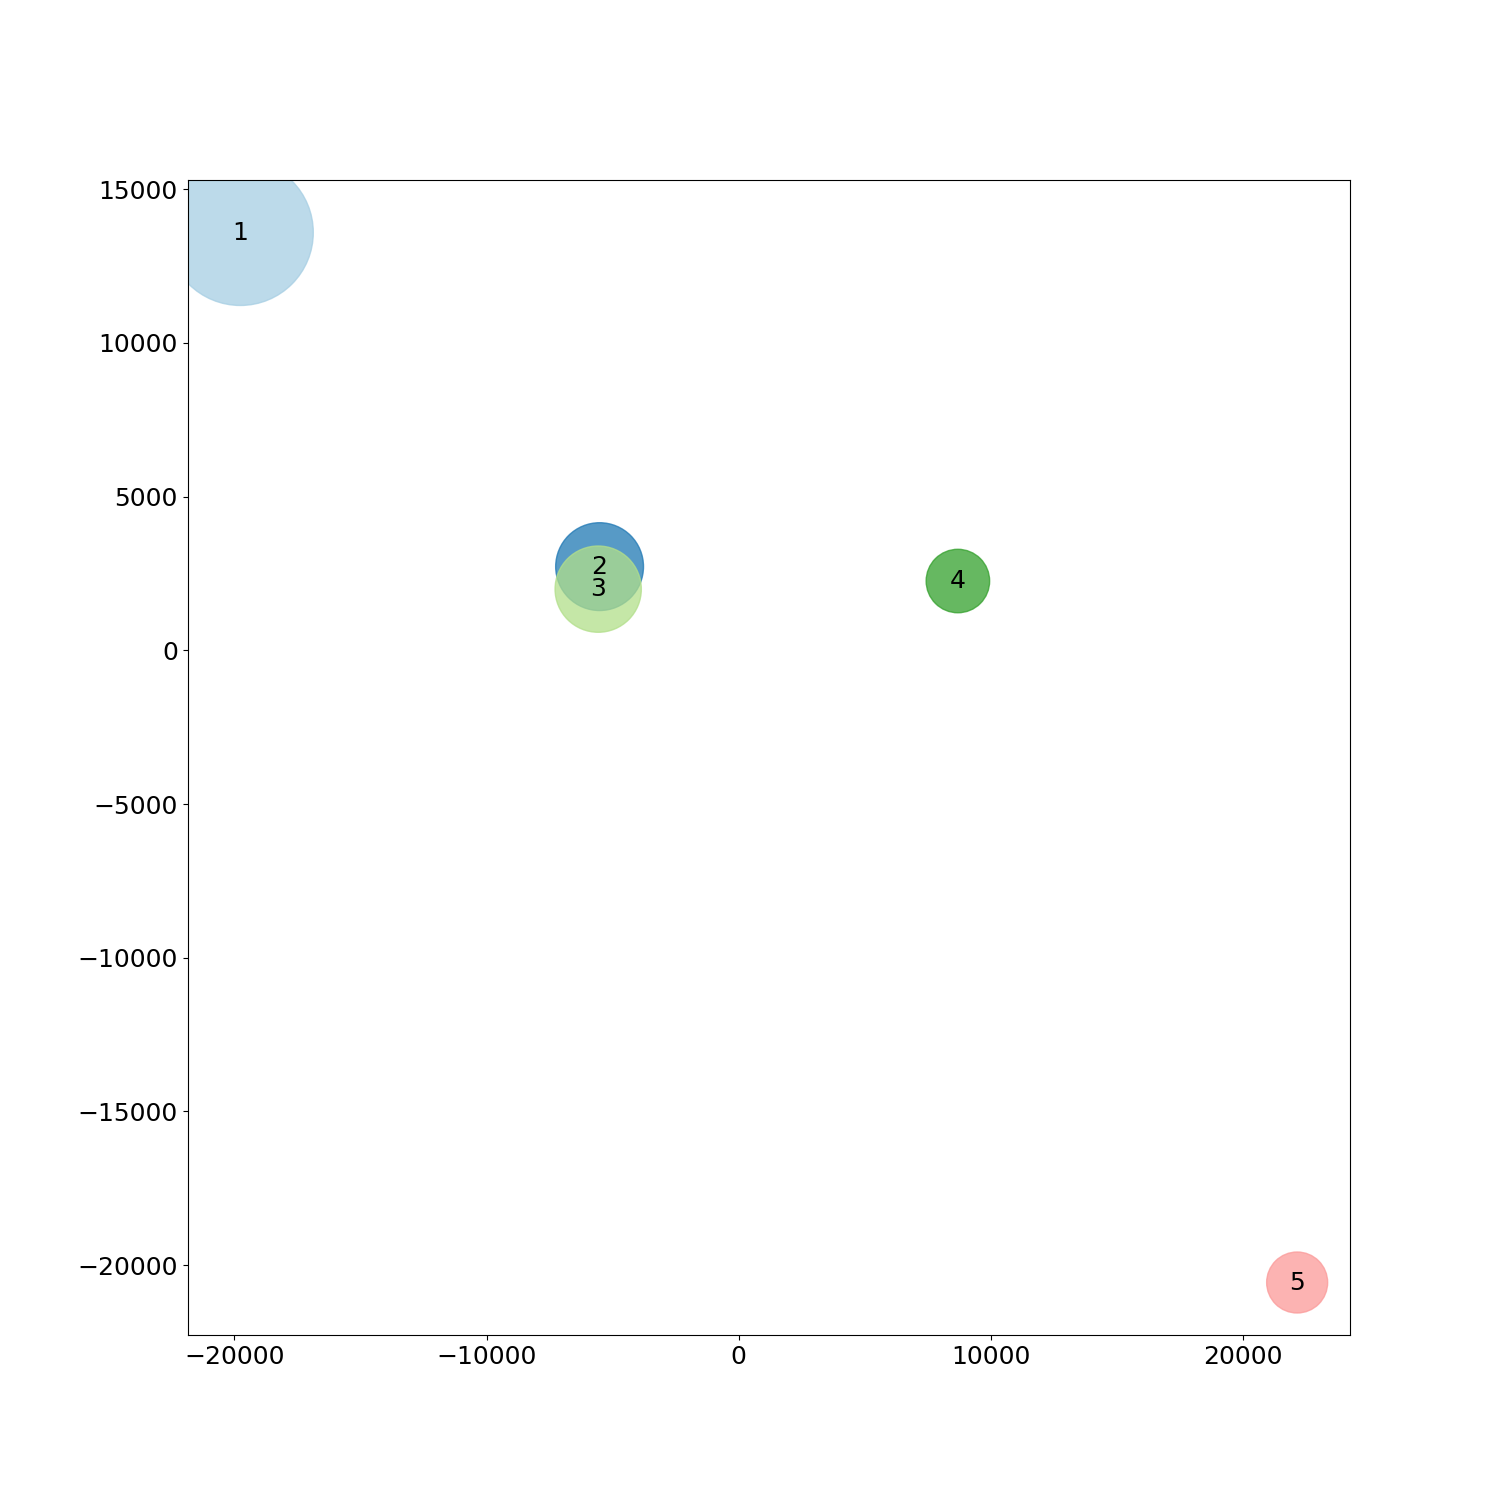
\includegraphics[scale=0.45]{caso2A/kmeans/mds.png}
\end{figure}

En \eqref{c2A_mds} se aprecia como los clusters están separados entre sí y tienen tamaños similares salvo por elc luster 5, que es de menor tamaño.

\begin{figure}[H]
\caption{Caso 2A - Parallel coordinates de kmeans}
\label{c2A_parallel}
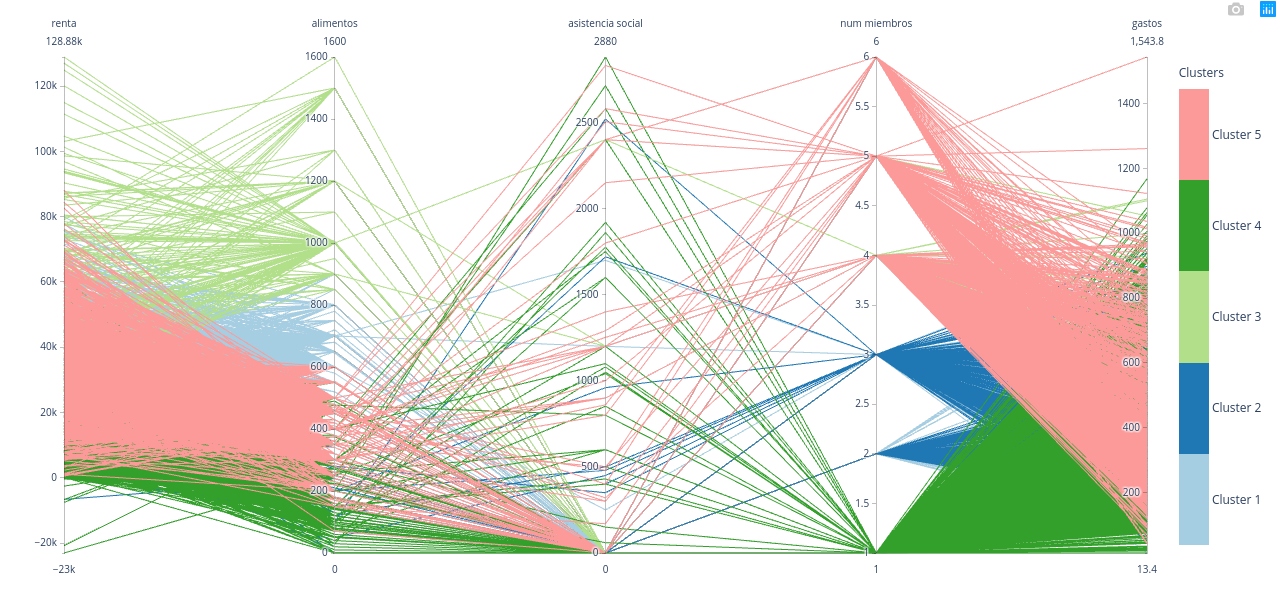
\includegraphics[scale=0.4]{caso2A/kmeans/parallel.png}
\end{figure}

En \eqref{c2A_parallel} se aprecia como el cluster verde claro, que alcanza mayores valores de asistencia social, es más disperso que los demás, lo que concuerda con la scatter matrix \eqref{c2A_scatter}. De nuevo, es claro que hay dos clusters que se diferencian por sus valores altos en alimentación y gastos.

En la tabla  \eqref{tab:c1_variables} se muestran qué variables son necesarias para identificar cada cluster:

\begin{table}[H]
\centering
\caption{Caso 1 - Variables necesarias para separar el clustering en spectral cluster}
\label{tab:c2A_variables}
\begin{tabular}{ccccc}
\toprule
 Cluster & renta & alimentos & asistencia social & gastos \\
\midrule
0 & & & & X \\
1 & X & & & X \\
2 & & X & & \\
3 & X & & & X \\
4 & & & X & \\
\bottomrule
\end{tabular}
\end{table}
Como se aprecia en \eqref{tab:c2A_variables} con una sola variable en cada cluster nos sirve para diferenciarlos entre los clusters 0, 2 y 4, mientras para los clusters 1 y 3 necesitamos dos para diferenciarlos entre ellos.

\subsection{Estudio de parámetros de DBSCAN}

Vamos a analizar el comportamiento de DBSCAN según sus parámetros principales. Para ello ejecutaremos la celda de parámetros de DBSCAN, que nos proporciona las medidas obtenidas para cada par de parámetros fijados.

\begin{table}[H]
\centering
\caption{Caso 2A - Cambio de parámetros DBSCAN}
\label{tab:c2A_dbscan}
\begin{tabular}{ccccccc}
\toprule
 Algoritmo & Tiempo (s) & Silhouette & Calinski-Harabasz & Número de clusters \\
\midrule
dbscan & 0.126 & 15.000 & 0.210 & 283.280 & 0.62692 & 2 \\
dbscan & 0.126 & 20.000 & 0.177 & 304.282 & 0.60850 & 2 \\
dbscan & 0.126 & 25.000 & 0.185 & 343.349 & 0.59182 & 2 \\
dbscan & 0.126 & 30.000 & 0.181 & 357.820 & 0.58212 & 2 \\
dbscan & 0.126 & 35.000 & 0.188 & 361.064 & 0.57576 & 2 \\
dbscan & 0.130 & 15.000 & 0.190 & 223.006 & 0.63128 & 2 \\
dbscan & 0.130 & 20.000 & 0.194 & 279.313 & 0.62217 & 2 \\
dbscan & 0.130 & 25.000 & 0.184 & 324.483 & 0.60954 & 2 \\
dbscan & 0.130 & 30.000 & 0.193 & 345.157 & 0.60186 & 2 \\
dbscan & 0.130 & 35.000 & 0.193 & 354.160 & 0.58156 & 2 \\
dbscan & 0.150 & 15.000 & 0.247 & 133.391 & 0.67010 & 2 \\
dbscan & 0.150 & 20.000 & 0.212 & 208.220 & 0.65089 & 2 \\
dbscan & 0.150 & 25.000 & 0.213 & 234.186 & 0.64523 & 2 \\
dbscan & 0.150 & 30.000 & 0.219 & 244.053 & 0.63871 & 2 \\
dbscan & 0.150 & 35.000 & 0.232 & 277.293 & 0.63108 & 2 \\
dbscan & 0.170 & 15.000 & 0.245 & 106.562 & 0.68737 & 2 \\
dbscan & 0.170 & 20.000 & 0.243 & 112.836 & 0.68127 & 2 \\
dbscan & 0.170 & 25.000 & 0.241 & 154.421 & 0.66746 & 2 \\
dbscan & 0.170 & 30.000 & 0.231 & 179.415 & 0.66353 & 2 \\
dbscan & 0.170 & 35.000 & 0.479 & 197.375 & 0.66118 & 2 \\
dbscan & 0.200 & 15.000 & 0.283 & 77.501 & 0.69224 & 2 \\
dbscan & 0.200 & 20.000 & 0.256 & 95.258 & 0.68918 & 2 \\
dbscan & 0.200 & 25.000 & 0.254 & 103.127 & 0.68949 & 2 \\
dbscan & 0.200 & 30.000 & 0.252 & 107.818 & 0.68620 & 2 \\
dbscan & 0.200 & 35.000 & 0.239 & 110.824 & 0.68431 & 2 \\
\bottomrule
\end{tabular}
\end{table}

Como podemos apreciar en \eqref{tab:c2A_dbscan} DBSCAN siempre realiza dos clusters. El tamaño de estos es siempre similar, más del $90\%$ los ejemplos están agrupados en el cluster $0$ y los restantes están en el $-1$.

Este algoritmo no ha hecho ninguna buena agrupación en ningún caso de los probados, pese a que su silhouette es bastante alto, lo que puede ser consecuencia de que los clusters estén muy separados.

No podemos interpretar demasiado Calinsk-Harabasz, ya que al no estar normalizado no sabemos si los valores dados son muy altos. Sí podemos decir que los mejores agrupamientos (que han proporcionado un valor de esta medida más alto) se han dado cuando min samples es $15$.


\subsection{Estudio de parámetros de Kmeans}

Estudiamos ahora el algoritmo Kmeans. Se ha variado el número de clusters.

\begin{table}[H]
\centering
\caption{Caso 2A - Cambio de parámetros Kmeans}
\label{tab:c2A_kmeans}
\begin{tabular}{cccccc}
\toprule
Algoritmo & n clusters & Tiempo(s) & Silhouette & Calinski-Harabasz & n clusters \\
\midrule
kmeans & 3.000 & 0.224 & 960.927 & 0.28417 & 3 \\
kmeans & 4.000 & 0.122 & 1162.049 & 0.31899 & 4 \\
kmeans & 5.000 & 0.283 & 1157.588 & 0.31325 & 5 \\
kmeans & 6.000 & 0.292 & 1174.483 & 0.32302 & 6 \\
kmeans & 7.000 & 0.328 & 1107.187 & 0.31675 & 7 \\
kmeans & 8.000 & 0.183 & 1074.974 & 0.31710 & 8 \\
kmeans & 9.000 & 0.487 & 1031.378 & 0.31904 & 9 \\
kmeans & 10.000 & 1.043 & 992.485 & 0.29012 & 10 \\
\bottomrule
\end{tabular}
\end{table}

Podemos ver en \eqref{tab:c2A_kmeans} que no hay demasiada diferencia entre las medidas obtenidas para los distintos valores del número de clusters, y destaca que el valor para el que se alcanza el máximo en Silhouette es el mismo para el que se alcanza el máximo en Calinski-harabasz, que es 6 clusters.

Aún así, kmeans ha dado resultados buenos en todos los casos y ha demostrado ser bastante robusto en sus agrupaciones.



\section{Interpretación de la segmentación}

A la vista de los resultados obtenidos, vemos que no se aprecian diferencias significativas en la renta entre las agrupaciones y no se encuentra demasiado dispersa. Esta variable por tanto no es tan relevante como otras.

No hay ninguna variable que destaque sobre otra, pero usando solamente las variables gastos, IRPF y alimentacion in podríamos diferenciar con claridad 3 clusters, y los otros dos agruparlos por descarte. Las otras variables nos sirvieron para refinar la diferenciación entre los clusters para lograr diferenciar los $5$.

Respecto a la hipótesis inicial, que las personas con propiedades alquiladas tienen mayor renta o más comodidades, en principio no parece cierta, pues la renta no ha sido una variable significativa respecto a la que dividir y otros factores son más influyentes.




